% !TEX TS-program = pdflatex
% !TEX encoding = UTF-8 Unicode

% This is a simple template for a LaTeX document using the "article" class.
% See "book", "report", "letter" for other types of document.

\documentclass[12pt]{article} % use larger type; default would be 10pt

\usepackage[utf8]{inputenc} % set input encoding (not needed with XeLaTeX)

%%% Examples of Article customizations
% These packages are optional, depending whether you want the features they provide.
% See the LaTeX Companion or other references for full information.

%%% PAGE DIMENSIONS
\usepackage{geometry} % to change the page dimensions
\geometry{a4paper} % or letterpaper (US) or a5paper or....
\geometry{margin=2.5cm} % for example, change the margins to 2 inches all round
% \geometry{landscape} % set up the page for landscape
%   read geometry.pdf for detailed page layout information

\usepackage{graphicx} % support the \includegraphics command and options

\usepackage[parfill]{parskip} % Activate to begin paragraphs with an empty line rather than an indent

\linespread{1.4}

%%% PACKAGES
\usepackage{booktabs} % for much better looking tables
\usepackage{array} % for better arrays (eg matrices) in maths
\usepackage{paralist} % very flexible & customisable lists (eg. enumerate/itemize, etc.)
\usepackage{verbatim} % adds environment for commenting out blocks of text & for better verbatim
\usepackage{subfig} % make it possible to include more than one captioned figure/table in a single float
\usepackage{times}
% These packages are all incorporated in the memoir class to one degree or another...

\usepackage{cite}
\usepackage{url} 

\usepackage{tikz}
\usepackage{tikzscale}
\usepackage{pgfplots}
\usepackage{pgfplotstable}

%%% HEADERS & FOOTERS
\usepackage{fancyhdr} % This should be set AFTER setting up the page geometry
\pagestyle{fancy} % options: empty , plain , fancy
\renewcommand{\headrulewidth}{0pt} % customise the layout...
\lhead{}\chead{}\rhead{}
\lfoot{}\cfoot{\thepage}\rfoot{}

%%% SECTION TITLE APPEARANCE
\usepackage{sectsty}
\allsectionsfont{\sffamily\mdseries\upshape} % (See the fntguide.pdf for font help)
% (This matches ConTeXt defaults)

%%% ToC (table of contents) APPEARANCE
\usepackage[nottoc,notlof,notlot]{tocbibind} % Put bibliography in the ToC
\usepackage[titles,subfigure]{tocloft} % Alter the style of the Table of Contents
\renewcommand{\cftsecfont}{\rmfamily\mdseries\upshape}
\renewcommand{\cftsecpagefont}{\rmfamily\mdseries\upshape} % No bold!

%%% END Article customizations

%%% The "real" document content comes below...

\title{ELEC2004 Design Challenge Report}
\author{
	{Ryan Fitzsimon}\\
	{43214907}\\
	\texttt{ryan.fitzsimon@uqconnect.edu.au}\\\\
	\and
	{Liam McMahon}\\
	{43186022}\\
	\texttt{liam.mcmahon1@uqconnect.edu.au}\\\\
}

%\date{} % Activate to display a given date or no date (if empty),
         % otherwise the current date is printed 

\begin{document}
\maketitle
\pagebreak





\section*{Abstract}
\cite{ProgPara}
\pagebreak





\tableofcontents
\pagebreak
\listoftables
\listoffigures
\pagebreak





\section{Introduction}
\subsection{Problem Description}

A black box containing a circuit of unknown composition was given for the group to analyse and design a reciprocal circuit which would negate the effects of the box. This meant that the desired output of the combination of the blackbox and the student designed circuit would be the same as the input into the combined circuits. 


The input signal to the circuit was a sinusoidal wave of 20V peak to peak, the frequency of which was between DC and 20 kHz. The only output load on the circuit was an oscilloscope of high impedance. The group was given three two hour sessions to design and test the proposed circuit, using a range of components supplied in the lab.



\subsection{Approach Taken}

The process of the design of the circuit involved several steps. First, the black box was analysed to find its transfer function. Once this had been determined, a circuit was designed to give the inverse of this transverse function so as to reverse the effects of the black box. The components that best matched the calculated requirements were then selected from the supplied components in the lab. Testing was then undertaken on the circuit to ensure that it worked as expected. Minor tweaks to the values of the components used were made to better satisfy the conditions of the project.

The circuit that best reversed the effects of the black box was a non inverting amplifier with a purely real feedback impedance and a complex dividing impedance. This circuit will be further explained later in the report.

\subsection{Report Breakdown}

This report will cover the following topics:
\begin{itemize} \itemsep1pt
	\item The background knowledge required to understand and replicate the results obtained;
	\item The experimental method used to obtain the results;
	\item The experimental results obtained;
	\item The design goals, method and outcome; and
	\item A discussion about the design process and outcome.
\end{itemize}

\pagebreak





\section{Background}

\subsection{Frequency Domain}

When a circuit involves energy storage components such as capacitors and inductors, it is often convenient to analyse a circuit in the frequency domain as opposed to the time domain. In order to analyse circuits in the frequency domain, each component's impedance must be known. Impedance is ratio of the voltage phasor through the component and the current phasor through the component. Figure 1 below shows the impedances of many common components.

\begin{figure}[h]
	\centering
	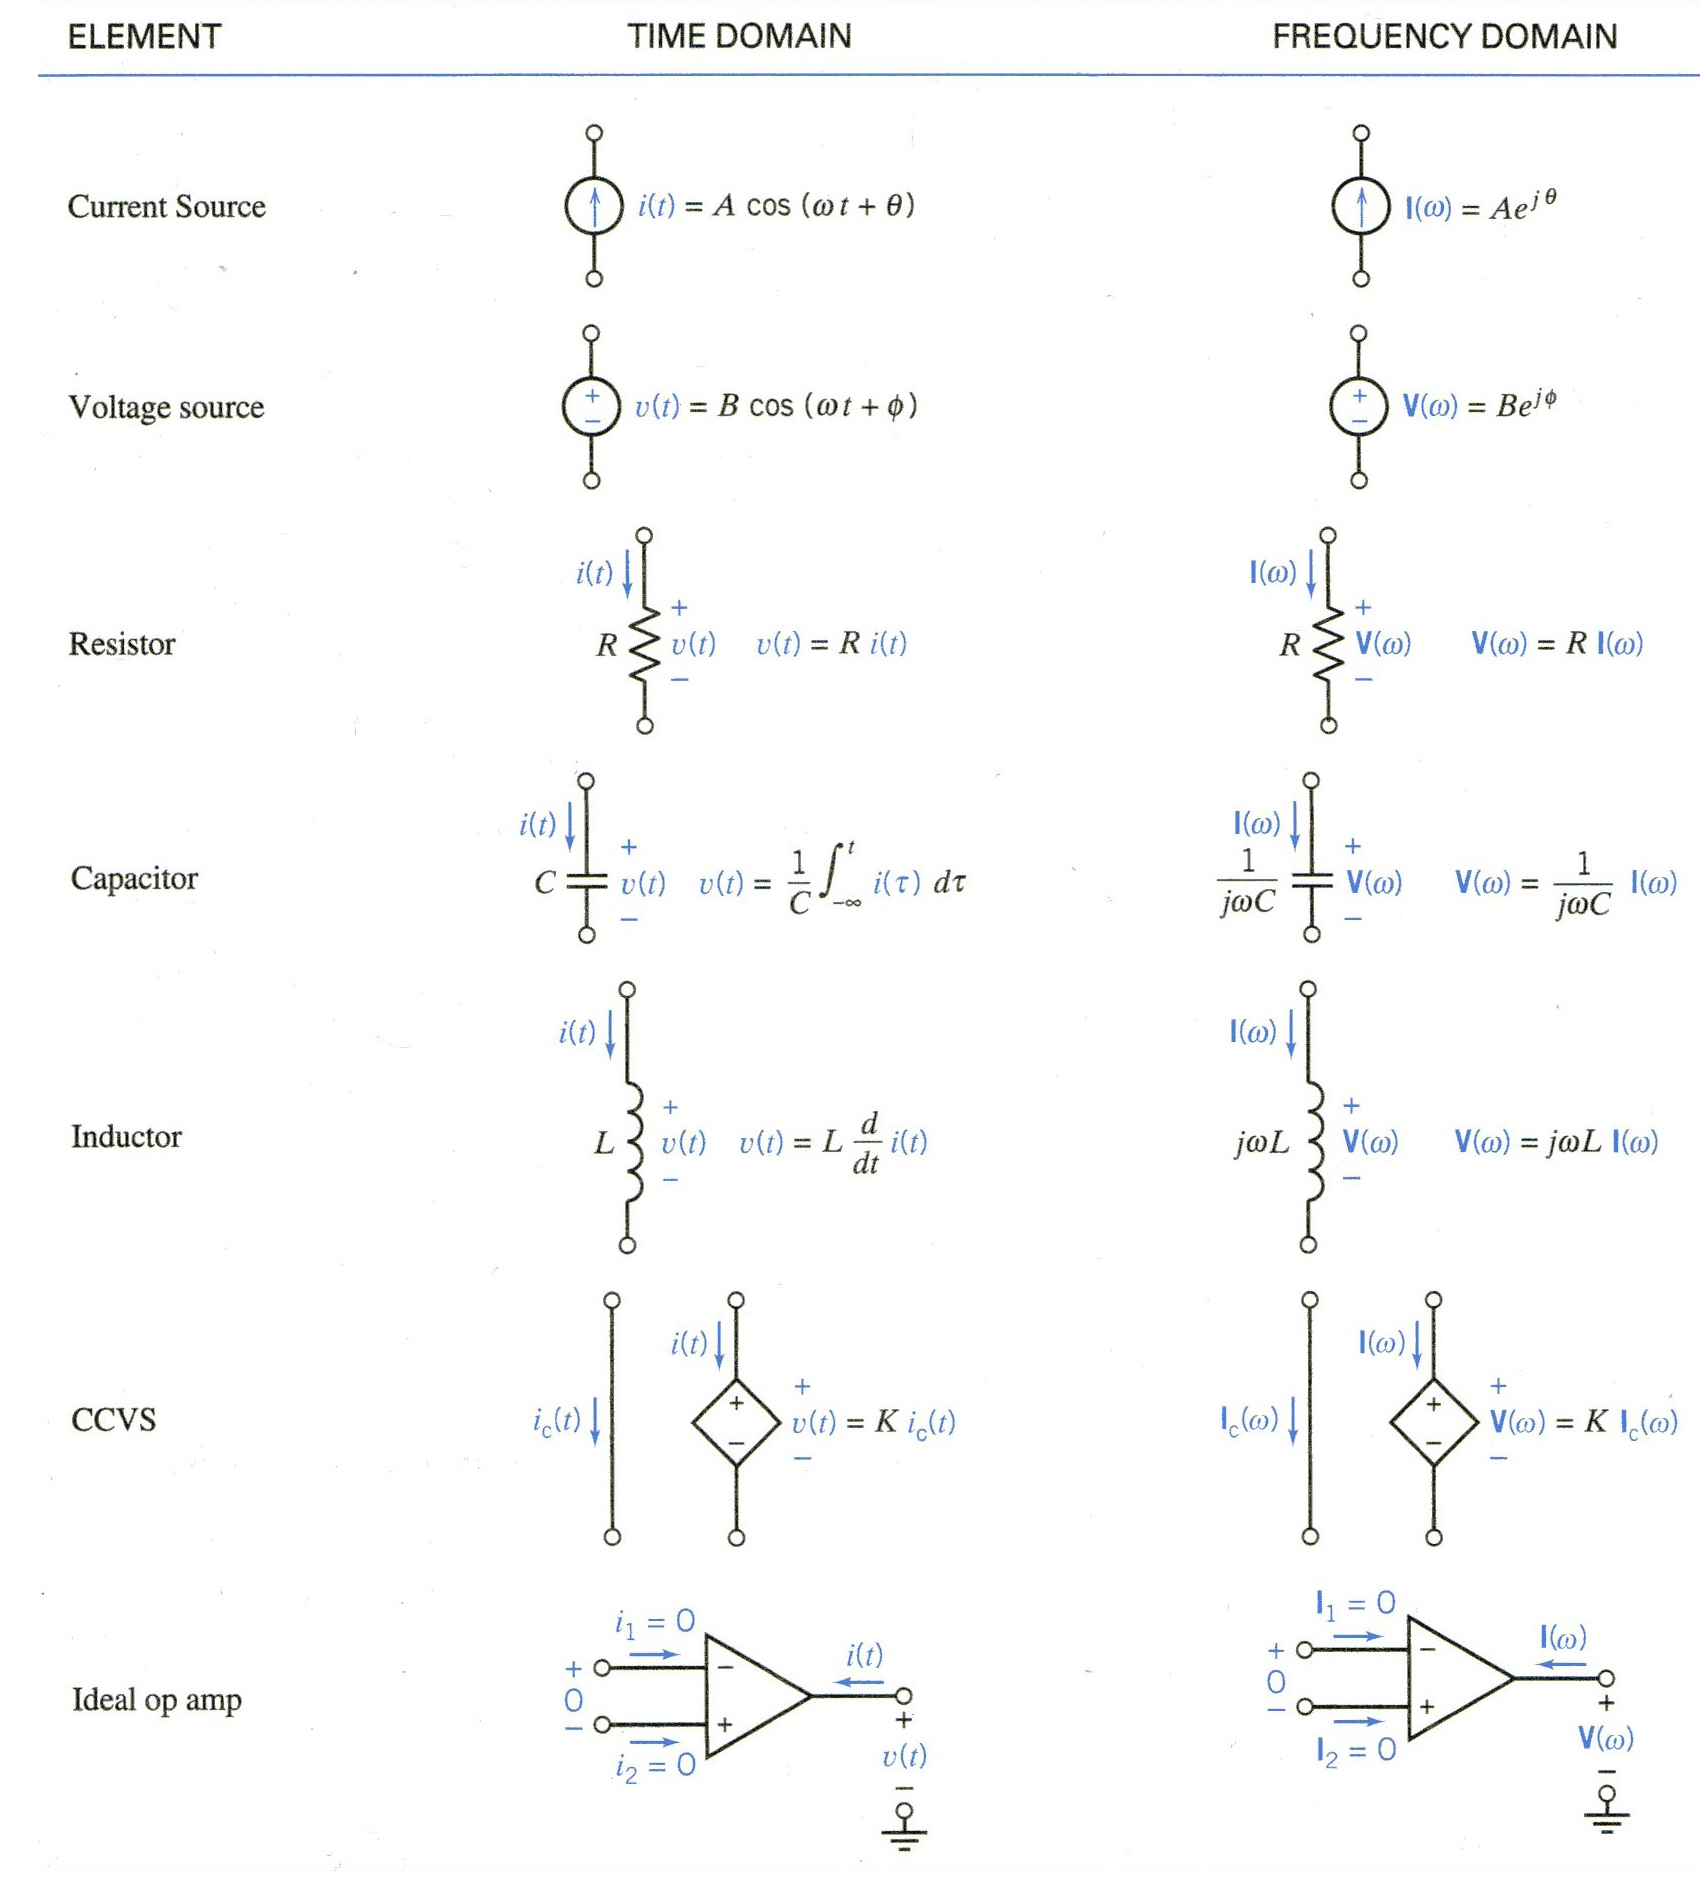
\includegraphics[scale=0.2]{Impedances1.jpg}
	\caption{List of common impedances (Dorf, R, Svoboda, J, 2014)}
\end{figure}



\subsection{Transfer Functions}

A transfer function is the ratio of the Laplace transform of the input to a circuit to the Laplace transform of the output. It is a useful tool for analysing circuits, as it allows the 

\textcolor{red}{poles and zeroes}

\pagebreak





\section{Experimental Method and Results}

\subsection{Analysing the Black Box}

\subsubsection{Experimental Method}

The apparatus used to analyse the black box was:
\begin{itemize} \itemsep1pt
	\item The black box;
	\item A wave generator; and
	\item An oscilloscope.
\end{itemize}


The properties of the wave generated by the wave generator was set using the oscilloscope to ensure they were known and suitable for use in the experiment. Specifically, the wave was set to be a sinusoidal wave with a peak to peak voltage of 20V and no offset.

The input of the black box was connected to the output of the wave generator. This input signal was also connected to one port of the oscilloscope to measure the voltage into the black box. The ground of the black box was connected to both the ground of the wave generator and the oscilloscope to ensure a constant reference. The output of the black box was connected to the input of the oscilloscope. 

Starting at a frequency of 1 Hertz, the input and output of the black box was recorded at regular intervals up to and including a frequency of 20 kiloHertz. This data can be seen and analysed in the following section of the report.

\subsubsection{Experimental Results}



\pagebreak

\subsection{Testing designed circuit}

\subsubsection{Experimental Method}

The apparatus used to test the designed circuit was:
\begin{itemize} \itemsep1pt
	\item The blackbox;
	\item The circuit;
	\item A wave generator; and
	\item An oscilloscope.
\end{itemize}


As with the analysis of the black box, the properties of the generated wave were set to be sinusoidal of peak to peak voltage of 20V and no offset.

The input of the black box was connected to the output of the wave generator. This input signal was also connected to one port of the oscilloscope to measure the voltage into the black box. The ground of the black box was connected to the ground of the wave generator, the ground of the oscilloscope and the ground of the designed circuit. The output of the black box was connected to the input of the designed circuit, and the output of this circuit was connected to the input of the oscilloscope.

Starting at a frequency of 1 Hertz, the input and output of the black box was recorded at regular intervals up to and including a frequency of 20 kiloHertz. This data can be seen and analysed in the following section of the report.

\subsubsection{Experimental Results}

\begin{figure}
 	\centering
	\includegraphics[width=\textwidth]{BlackBox.tikz}
	\caption{Blackbox}
\end{figure}

\begin{figure}
 	\centering
	\includegraphics[width=\textwidth]{Designed.tikz}
	\caption{Designed}
\end{figure}

\begin{figure}
 	\centering
	\includegraphics[width=\textwidth]{Combined.tikz}
	\caption{Combined}
\end{figure}

\pagebreak





\section{Design}

\subsection{Goals}


\subsection{Method}


\subsection{Outcomes}
\pagebreak





\section{Discussion}

As can be seen from Figure 4, the designed circuit was very effective at negating the black box. The only weakness in the design was the slight dip in the gain at mid range frequencies, and the smaller drop at high frequencies. However, the maximum deviation of the actual output from the expected was -1.6dB, which is very small considering the simplicity of the design. It can be seen that in the Bode plot of the designed circuit that the actual values of the zeroes and poles do not quite match up with the expected values \textcolor{red}{(I'll put legit values in here)} and this is what is causing the descrepencies. This could have been avoided by selecting more components to be placed in series and/or parallel with the chosen ones to make the values more accurately match up with the ideal calculated ones.

The experiments were carried out to the highest degree of accuracy possible with the given equiment and time constraints. Where measurements were taken that appeared to be sensitive to small changes, the values were checked several times. Sufficient data was collected to thoroughly analyse the blackbox, and this helped greatly with the process of design of the negation circuit. From the data

\pagebreak





\section{Conclusion}
\pagebreak




\section{Bibliography}
\bibliographystyle{ieeetr}
\bibliography{DesignChallengeReport}
\pagebreak





\section{Appendices}


\begin{table}[htb]
	\begin{center}
		\pgfplotstabletypeset[col sep=tab]{Combined.dat}
	\end{center}
	\caption{Combined}
\end{table}

\begin{table}[htb]
	\begin{center}
		\pgfplotstabletypeset[col sep=tab]{BlackBox.dat}
	\end{center}
	\caption{BlackBox}
\end{table}

\begin{table}[htb]
	\begin{center}
		\pgfplotstabletypeset[col sep=tab]{Designed.dat}
	\end{center}
	\caption{Designed}
\end{table}



\end{document}
